\documentclass[10pt]{beamer} 
     \hypersetup{pdfpagemode=FullScreen} 
     \usepackage{tikz} 
     \usetikzlibrary{shadows,patterns,shapes} 
     \usetikzlibrary{shapes.arrows,chains} 
     % serifenfreier Font -- fuer Praesentation geeignet/er 
     \listfiles % damit im Log alle benutzten Pakete aufgelistet werden 
     \usetheme[progressbar=frametitle]{metropolis} 
     \usepackage{appendixnumberbeamer} 
     \usepackage{booktabs} 
     \usepackage[scale=2]{ccicons} 
     \usepackage[utf8]{inputenc} 
     \usepackage{pgfplots} 
     \usepgfplotslibrary{dateplot} 
     \usepackage[ngerman]{babel} 
     \usepackage{xspace} 
     \usebackgroundtemplate{
     \tikz[overlay,remember picture] 
     \node[opacity=0.3, at=(current page.south east),anchor=south east,inner sep=0pt] {
     
\includegraphics[width=1.53\textwidth]{./PDFcreater/Pictures/background.png}};
     } 
     %\usebackgroundtemplate{
\includegraphics[,right]{./PDFcreater/Pictures/background.png}}
     \definecolor{Purple}{HTML}{6D087C}
     \definecolor{Orange}{HTML}{CF4A30}
     
     % Theme colors are derived from these two elements
     \setbeamercolor{alerted text}{fg=Orange}
     
     % ... however you can of course override styles of all elements 
     \setbeamercolor{frametitle}{bg=Purple}
     
     \title{Feedback der Studierenden im Kurs: Nx } 
     \begin{document} 
     \maketitle 
\begin{frame}[fragile]{1Geschlecht der Studis} 
 \begin{figure}
 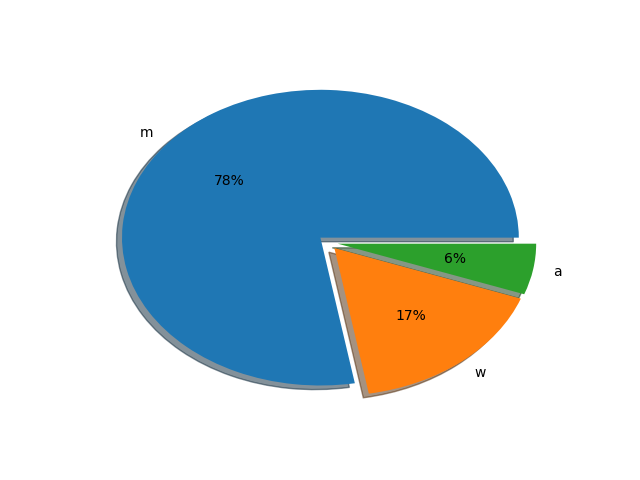
\includegraphics[width= 0.9\linewidth]{./PDFcreater/Plots/Nx/1Geschlecht+der+Studis.png};
 \end{figure}
 \end{frame}
\begin{frame}[fragile]{1Studiengang der Studis} 
 \begin{figure}
 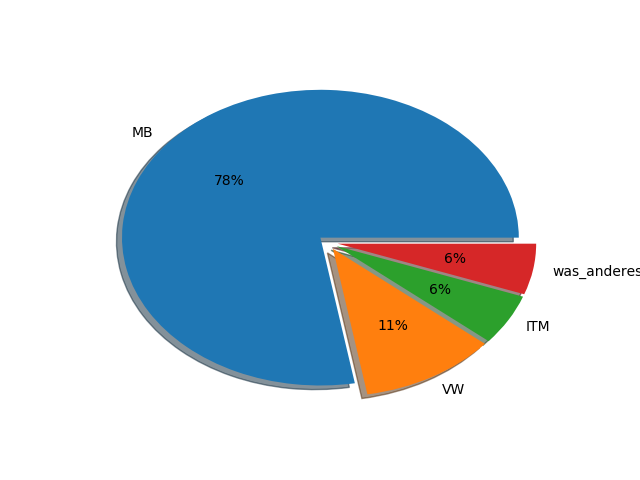
\includegraphics[width= 0.9\linewidth]{./PDFcreater/Plots/Nx/1Studiengang+der+Studis.png};
 \end{figure}
 \end{frame}
\begin{frame}[fragile]{1Tutor der Studis} 
 \begin{figure}
 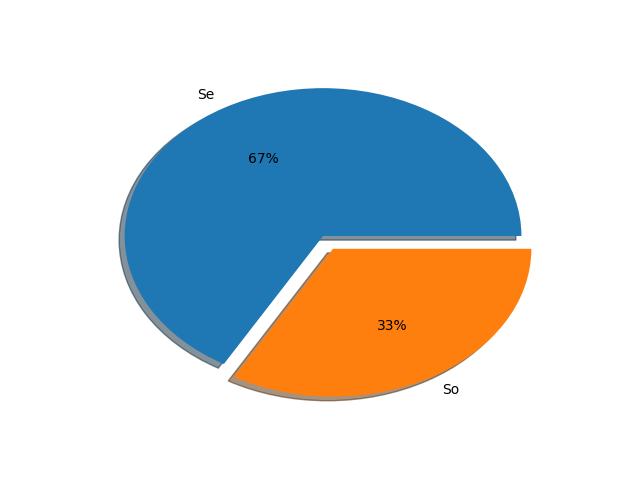
\includegraphics[width= 0.9\linewidth]{./PDFcreater/Plots/Nx/1Tutor+der+Studis.png};
 \end{figure}
 \end{frame}
\begin{frame}[fragile]{Benoetigte Stundenzahl vom gesamten CAD Kurs pro Woche} 
 \begin{figure}
 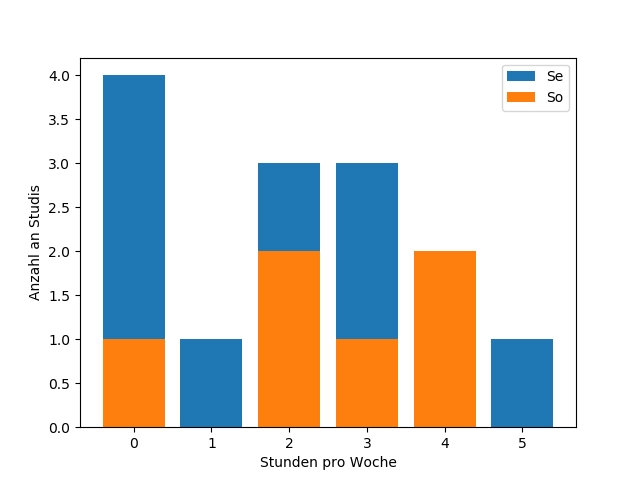
\includegraphics[width= 0.9\linewidth]{./PDFcreater/Plots/Nx/Benoetigte+Stundenzahl+vom+gesamten+CAD+Kurs+pro+Woche.png};
 \end{figure}
 \end{frame}
\begin{frame}[fragile]{Der Lehrinhalt war ausreichend um die HA zu bearbeiten} 
 \begin{figure}
 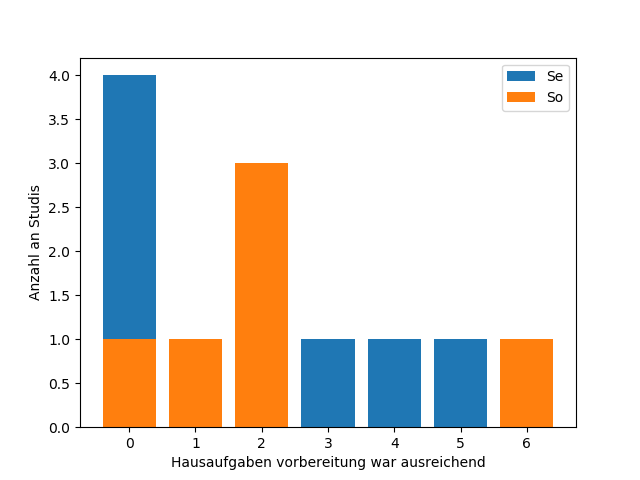
\includegraphics[width= 0.9\linewidth]{./PDFcreater/Plots/Nx/Der+Lehrinhalt+war+ausreichend+um+die+HA+zu+bearbeiten.png};
 \end{figure}
 \end{frame}
\begin{frame}[fragile]{Der Schwierigkeitsgrad war hoch} 
 \begin{figure}
 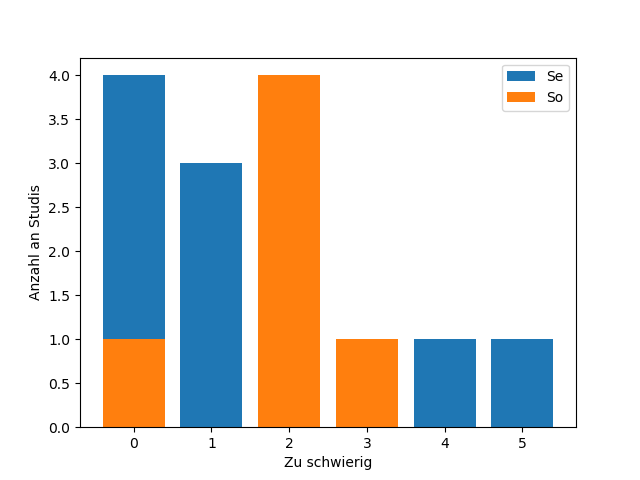
\includegraphics[width= 0.9\linewidth]{./PDFcreater/Plots/Nx/Der+Schwierigkeitsgrad+war+hoch.png};
 \end{figure}
 \end{frame}
\begin{frame}[fragile]{Die Formulierungen in der Hausaufgabe waren eindeutig} 
 \begin{figure}
 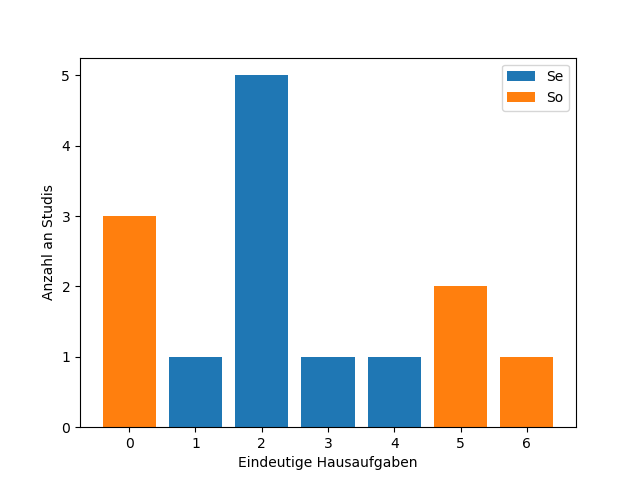
\includegraphics[width= 0.9\linewidth]{./PDFcreater/Plots/Nx/Die+Formulierungen+in+der+Hausaufgabe+waren+eindeutig.png};
 \end{figure}
 \end{frame}
\begin{frame}[fragile]{Die Hausaufgabe sollte vom Umfang her reduziert werden} 
 \begin{figure}
 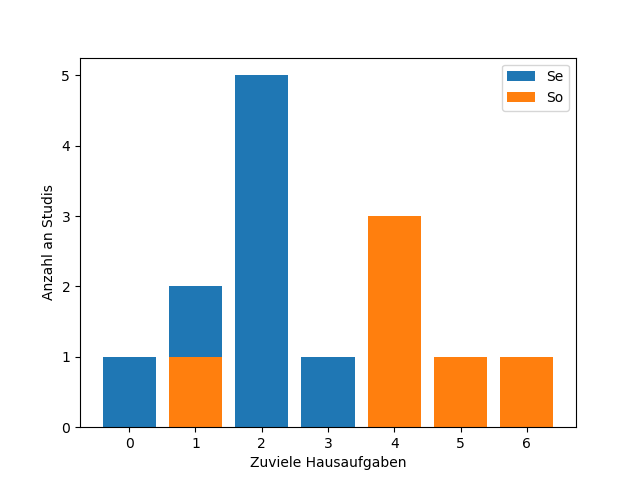
\includegraphics[width= 0.9\linewidth]{./PDFcreater/Plots/Nx/Die+Hausaufgabe+sollte+vom+Umfang+her+reduziert+werden.png};
 \end{figure}
 \end{frame}
\begin{frame}[fragile]{Die Uebungen sind gut strukturiert} 
 \begin{figure}
 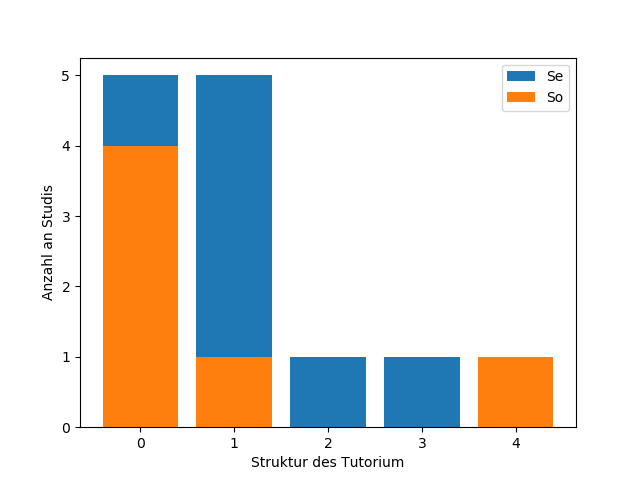
\includegraphics[width= 0.9\linewidth]{./PDFcreater/Plots/Nx/Die+Uebungen+sind+gut+strukturiert.png};
 \end{figure}
 \end{frame}
\begin{frame}[fragile]{Die Uebungsbeispiele sind gut gewaehlt} 
 \begin{figure}
 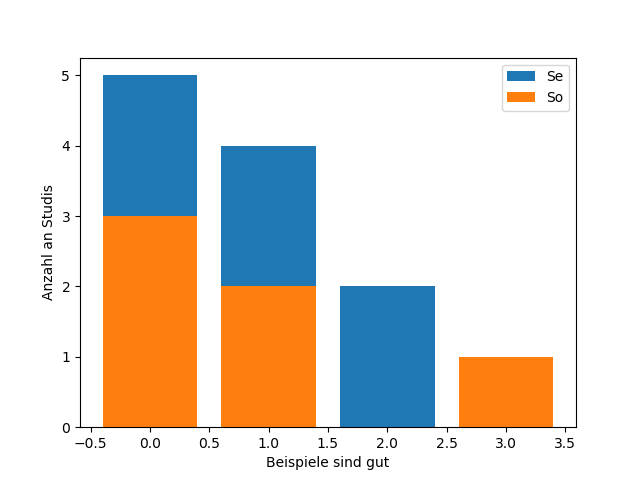
\includegraphics[width= 0.9\linewidth]{./PDFcreater/Plots/Nx/Die+Uebungsbeispiele+sind+gut+gewaehlt.png};
 \end{figure}
 \end{frame}
\begin{frame}[fragile]{Ich habe die Uebungsaufgaben alle gemacht} 
 \begin{figure}
 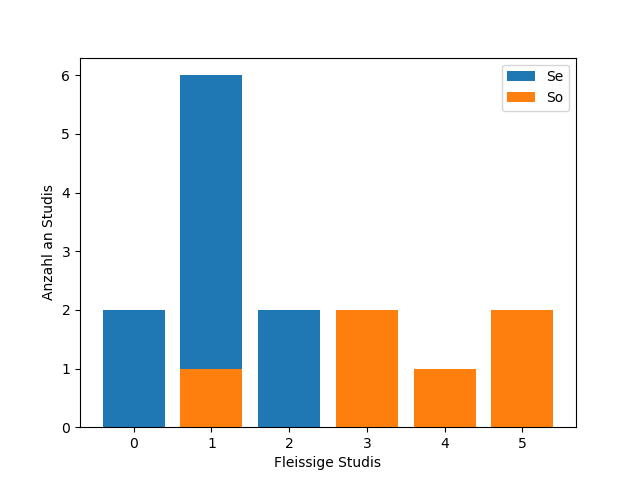
\includegraphics[width= 0.9\linewidth]{./PDFcreater/Plots/Nx/Ich+habe+die+Uebungsaufgaben+alle+gemacht.png};
 \end{figure}
 \end{frame}
\begin{frame}[fragile]{Ich habe mich schon fruehzeitig mit dem Programm zu Hause beschaeftigt} 
 \begin{figure}
 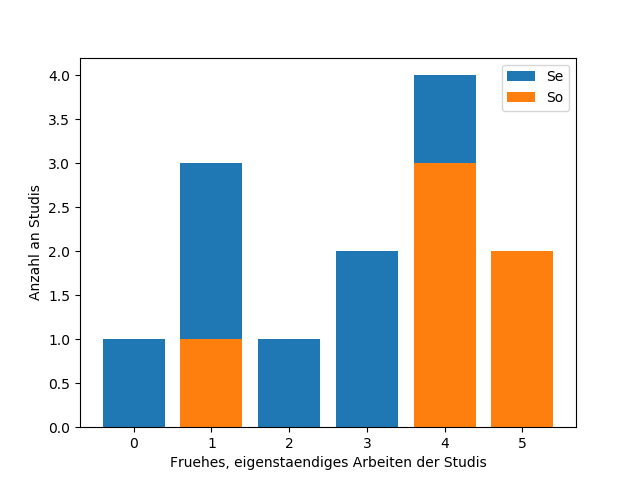
\includegraphics[width= 0.9\linewidth]{./PDFcreater/Plots/Nx/Ich+habe+mich+schon+fruehzeitig+mit+dem+Programm+zu+Hause+beschaeftigt.png};
 \end{figure}
 \end{frame}
\begin{frame}[fragile]{Ich habe viel Zeit zur Bearbeitung der Hausaufgabe benoetigt} 
 \begin{figure}
 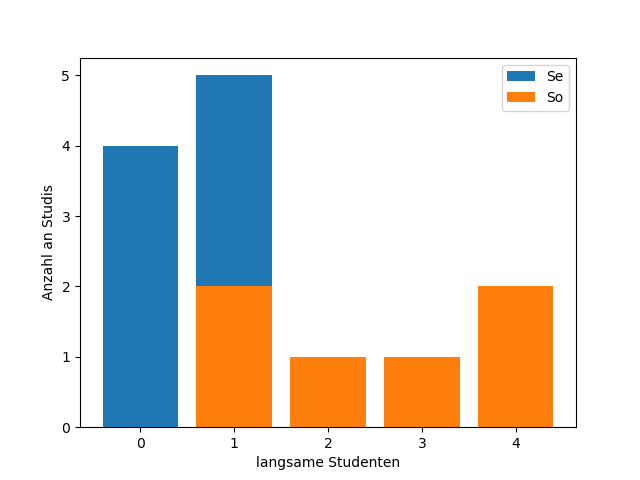
\includegraphics[width= 0.9\linewidth]{./PDFcreater/Plots/Nx/Ich+habe+viel+Zeit+zur+Bearbeitung+der+Hausaufgabe+benoetigt.png};
 \end{figure}
 \end{frame}
\begin{frame}[fragile]{Ich haette gerne mehr Uebungsaufgaben gehabt} 
 \begin{figure}
 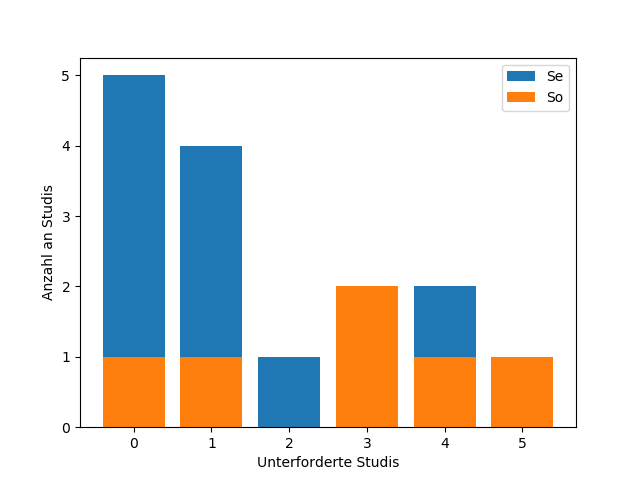
\includegraphics[width= 0.9\linewidth]{./PDFcreater/Plots/Nx/Ich+haette+gerne+mehr+Uebungsaufgaben+gehabt.png};
 \end{figure}
 \end{frame}
\begin{frame}[fragile]{Ich war immer gut auf das Tutorium vorbereitet} 
 \begin{figure}
 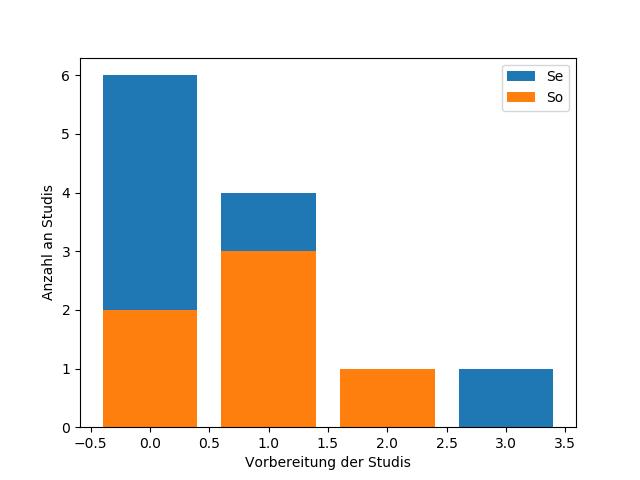
\includegraphics[width= 0.9\linewidth]{./PDFcreater/Plots/Nx/Ich+war+immer+gut+auf+das+Tutorium+vorbereitet.png};
 \end{figure}
 \end{frame}
\begin{frame}[fragile]{Semester der Studierenden} 
 \begin{figure}
 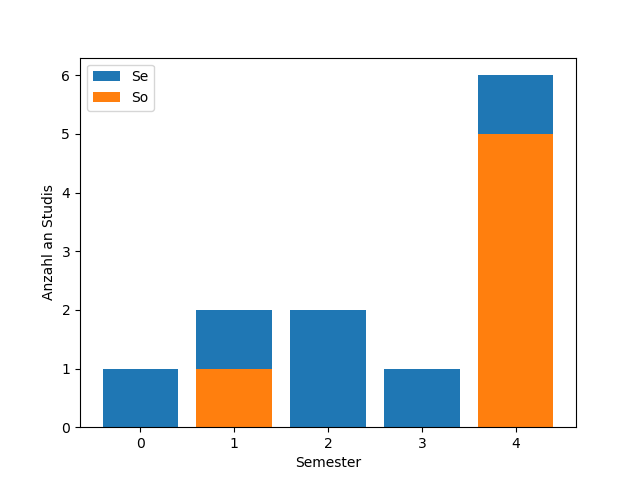
\includegraphics[width= 0.9\linewidth]{./PDFcreater/Plots/Nx/Semester+der+Studierenden.png};
 \end{figure}
 \end{frame}
\begin{frame}[fragile]{Tutor foerdert aktive Teilnahme der Studenten} 
 \begin{figure}
 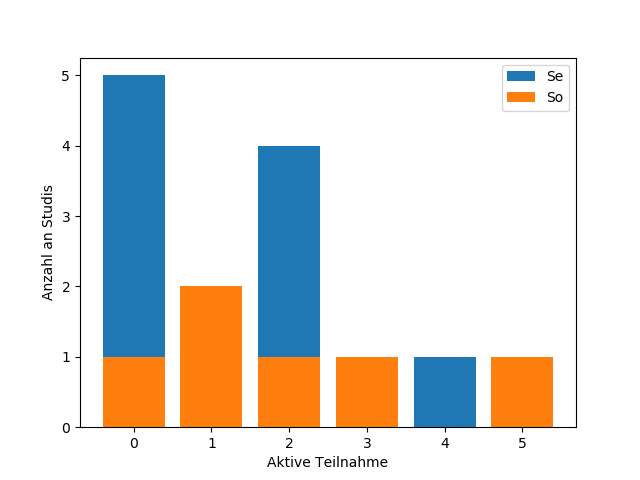
\includegraphics[width= 0.9\linewidth]{./PDFcreater/Plots/Nx/Tutor+foerdert+aktive+Teilnahme+der+Studenten.png};
 \end{figure}
 \end{frame}
\begin{frame}[fragile]{Tutor ist immer gut auf das Tutorium vorbereitet} 
 \begin{figure}
 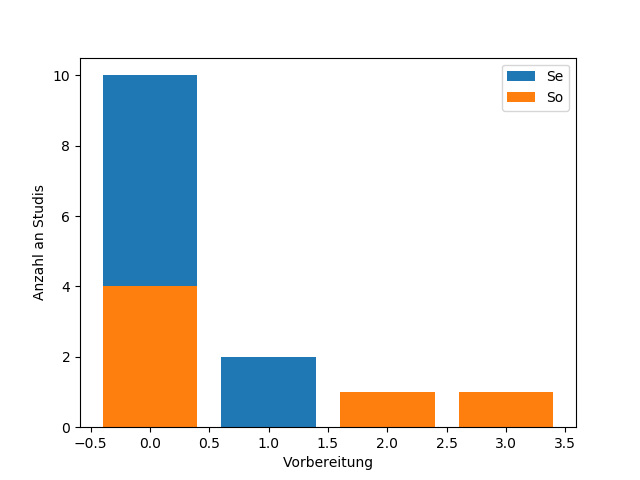
\includegraphics[width= 0.9\linewidth]{./PDFcreater/Plots/Nx/Tutor+ist+immer+gut+auf+das+Tutorium+vorbereitet.png};
 \end{figure}
 \end{frame}
\begin{frame}[fragile]{Tutor kann den Lehrinhalt verstaendlich darlegen} 
 \begin{figure}
 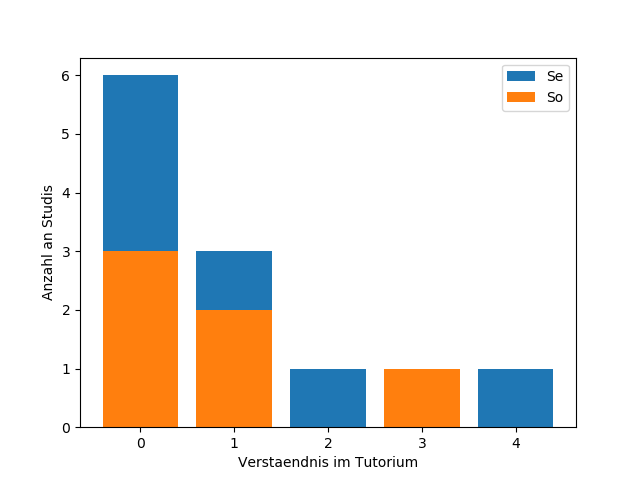
\includegraphics[width= 0.9\linewidth]{./PDFcreater/Plots/Nx/Tutor+kann+den+Lehrinhalt+verstaendlich+darlegen.png};
 \end{figure}
 \end{frame}
\begin{frame}[fragile]{Kommmentare der Studenten, Tutor: Se}Eine Stunde Zeit reicht oft nicht.Besser wäre 1.30 Stunde pro Woche zu haben.;
 \end{frame}
\begin{frame}[fragile]{Kommmentare der Studenten, Tutor: Se}die PCs im PC Pool laufen langsam. ;
 \end{frame}
\begin{frame}[fragile]{Kommmentare der Studenten, Tutor: Se}Anrechnung mit ECTS Punkten wäre wünschenswert;
 \end{frame}
\begin{frame}[fragile]{Kommmentare der Studenten, Tutor: Se}Falls die Bahn Verspätung hatte und man deswegen zu spät kam, war es manchmal etwas schwierig, dann noch in das Tutorium einsteigen zu können. In manchen Übungen waren Dokumente mit den ersten Zwischenschritten gespeichert, sodass amn auch später gut einsteigen konnte.;
 \end{frame}
\begin{frame}[fragile]{Kommmentare der Studenten, Tutor: Se}Der kurs ist im ganzen echt gut. Ich fände es nur 
 besser wenn die Hausaufgaben wie in Solid Edge gehalten wäre.(Eine große über das ganze Semester);
 \end{frame}
\begin{frame}[fragile]{Kommmentare der Studenten, Tutor: Se}Ich finde es sehr gut, dass solch eine Einführung in ein CAD Programm angeboten wird. Das erleichtert einem den Einstieg, auch wenn natürlich nicht alle Möglichkeiten des Programms in der kurzen Zeit gezeigt werden können. Es hat mir auch gefallen, dass auf Probleme in der Übung direkt eingegangen wurde.;
 \end{frame}
\begin{frame}[fragile]{Kommmentare der Studenten, Tutor: So}mehr Inhalt!;
 \end{frame}
\begin{frame}[fragile]{Kommmentare der Studenten, Tutor: So}Finde ich super, dass der Kurs angeboten wird. Hat mir für K2 sehr geholfen. Für mich war das Niveau sehr angemessen. 
 Ich würde es gut finden, wenn man von zu hause mehr Möglichkeiten hätte, die Tutoren zu erreichen. MailAdressen oder ein Forum bei Isis oder sowas. Ich hatte in den Ferien ein Problem und konnte es erst lösen, als ich wieder in der uni war.;
 \end{frame}
\begin{frame}[fragile]{Kommmentare der Studenten, Tutor: Se}Alles gut :D Hausaufgaben nicht gemacht, ich hoffe man besteht auch ohne ;);
 \end{frame}
\begin{frame}[fragile]{Kommmentare der Studenten, Tutor: So}Alles schick, vllt. ein paar Beispiele die für die K2 Hausaufgabe sinnvoll sind, wie Constantin es letztes Semester gemacht hat.. also frühzeitig was zur Zeichnungsableitung, evtl. Tipps zu Gehäusegestaltung und größere Baugruppen usw.
 Dankeschön <3;
 \end{frame}
\begin{frame}[fragile]{Kommmentare der Studenten, Tutor:So}Sehr guter Kurs;
 \end{frame}
\end{document}